\subsubsection{Red LED Parallel Port}

The red lights {\it LEDR}$_{9-0}$ on the \DEBoard~board
are driven by an output parallel port, as illustrated in Figure \ref{fig:LED_port}. The port
contains a 10-bit {\it Data} register, which has the
address {\sf 0xFF200000}.  This register can be written or read by the processor using word 
accesses, and the upper bits not used in the registers are ignored.

\begin{figure}[h!]
   \begin{center}
       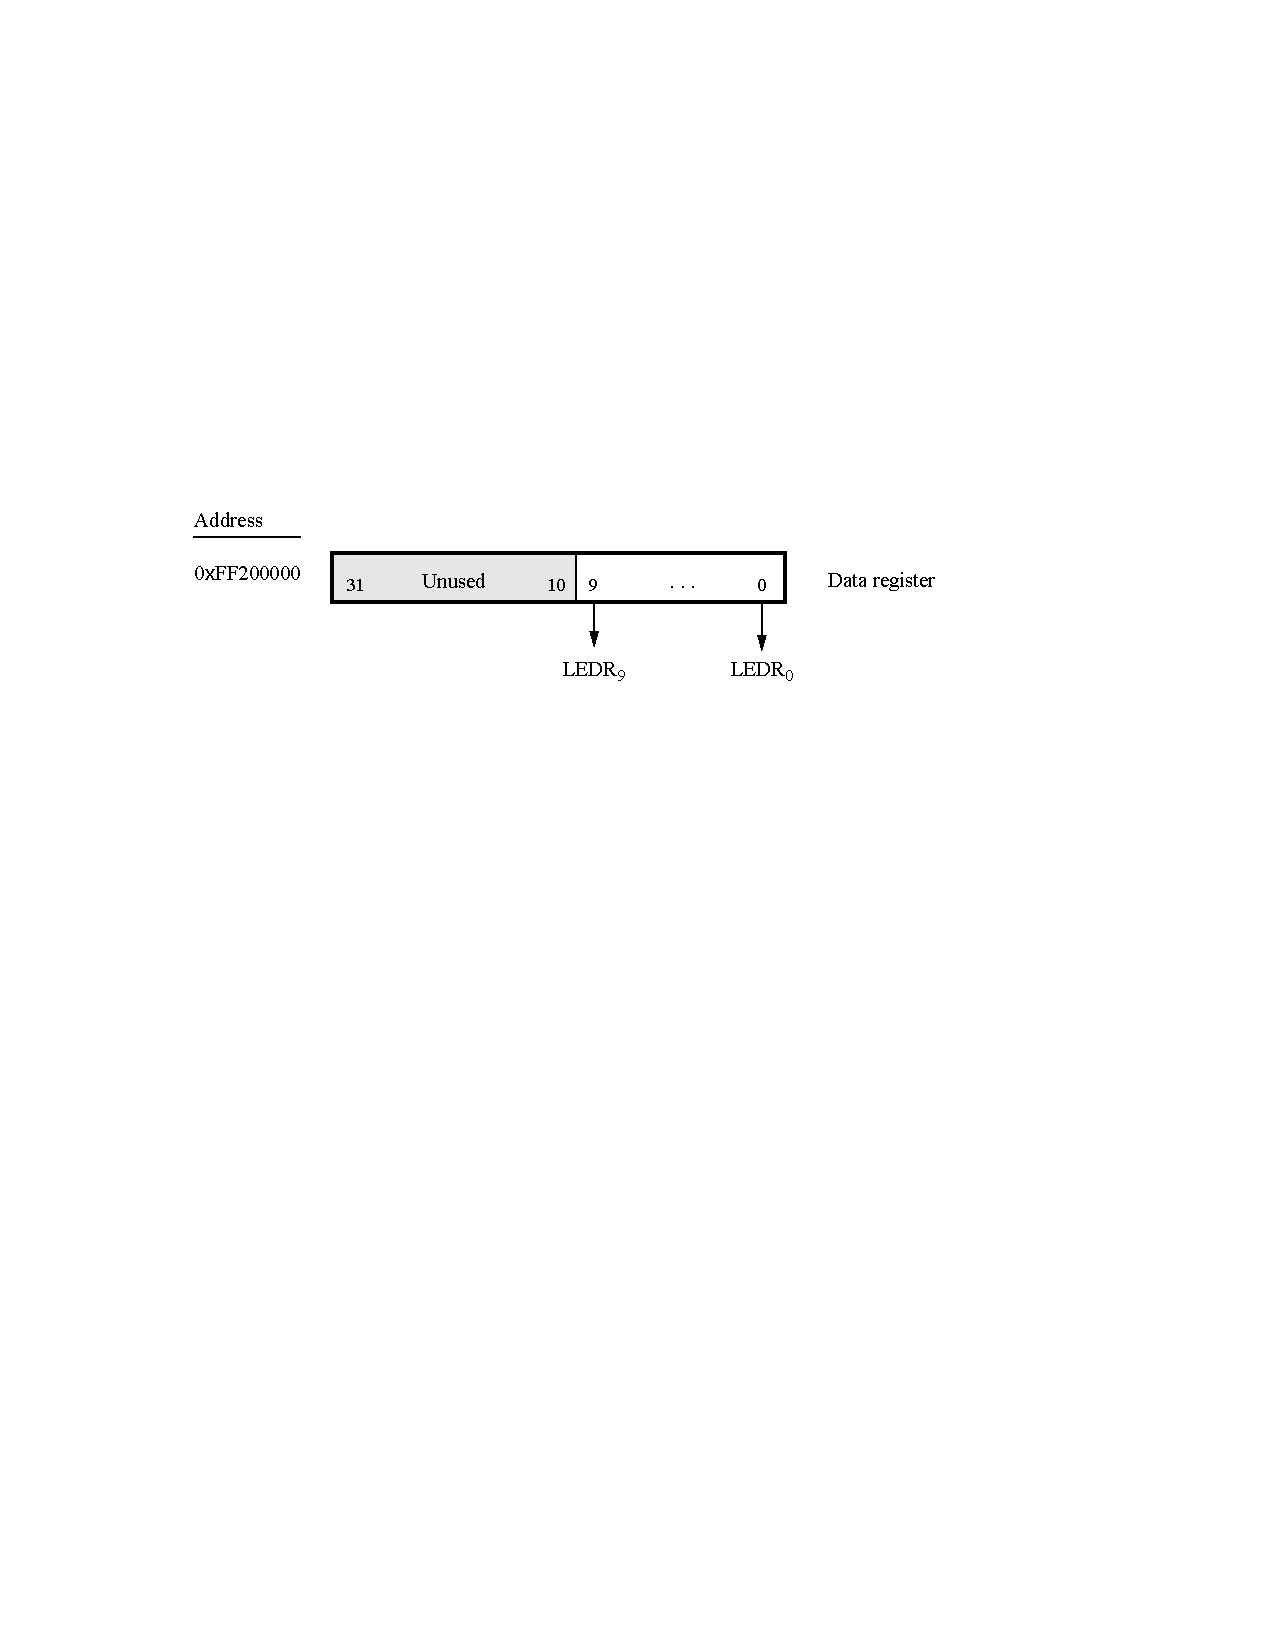
\includegraphics{../../../common/figs/FPGA_PP_Red_LEDs_10.pdf}
   \end{center}
   \caption{Output parallel port for {\it LEDR}.}
	\label{fig:LED_port}
\end{figure}


